\section{Preventivo}
	In questa sezione verranno riportati i preventivi per le varie fasi di lavoro, considerando che la fasi di analisi e consolidamento dei requisiti non verranno rendicontate nel preventivo finale. 
	La suddivisione oraria dei ruoli per ogni membro del gruppo dovrà rispettare le seguenti regole:
		\begin{itemize}
		\item ogni componente dovrà ricoprire almeno una volta ogni ruolo e per almeno otto ore;
		\item le ore lavorative totali per ogni fase dovranno essere le stesse per ogni componente.
	\end{itemize}
	 Per facilitare la comprensione dei ruoli nelle tabelle, essi verranno abbreviati con le seguenti sigle identificative:
			\begin{itemize}
			\item\textbf{Re:} responsabile;
			\item\textbf{Am:} amministratore;
			\item\textbf{An:} analista;
			\item\textbf{Pg:} progettista;
			\item\textbf{Pr:} programmatore;
			\item\textbf{Ve:} verificatore.
		\end{itemize}
	
	
	
	\subsection{Fase di analisi dei requisiti}
		\subsubsection{Prospetto orario}
			Durante la fase di analisi dei requisiti la distribuzione oraria preventivata dei ruoli di ogni componente del gruppo sarà la seguente:
			
			\rowcolors{2}{white}{lightest-grayest}
			\begin{longtable}{|c|c|c|c|c|c|c|c|}
				\hline
				\rowcolor{lighter-grayer}
				\textbf{Nome} & \textbf{Re} & \textbf{Am} & \textbf{An} & \textbf{Pg}  & \textbf{Pr}   & \textbf{Ve} & \textbf{Totale} \\
				\hline
				\endfirsthead
				
				\hline
				Giuseppe Vito Bitetti & 0 & 9 & 9 & 0 & 0 & 12 & 30\\
				\hline
				\hline
				Lorenzo Dei Negri & 8 & 0 & 13 & 0 & 0 & 9 & 30\\
				\hline
				\hline
				Nicolò Frison & 0 & 10 & 8 & 0 & 0 & 12 & 30\\
				\hline
				\hline
				Fouad Mouad & 0 & 7 & 11 & 0 & 0 & 12 & 30\\
				\hline
				\hline
				Mariano Sciacco & 8 & 0 & 12 & 0 & 0 & 10 & 30\\
				\hline
				\hline
				Alessandro Tommasin & 11 & 0 & 10 & 0 & 0 & 9 & 30\\
				\hline
				\hline
				Giovanni Vidotto & 0 & 7 & 8 & 0 & 0 & 15 & 30\\
				\hline 
				\caption{Tabella contenente il prospetto orario preventivato per la fase di analisi dei requisiti}
			\end{longtable}
			\pagebreak
		
			La tabella può essere riassunta nel seguente istogramma:
		
			\begin{figure}[H]
				\centering
				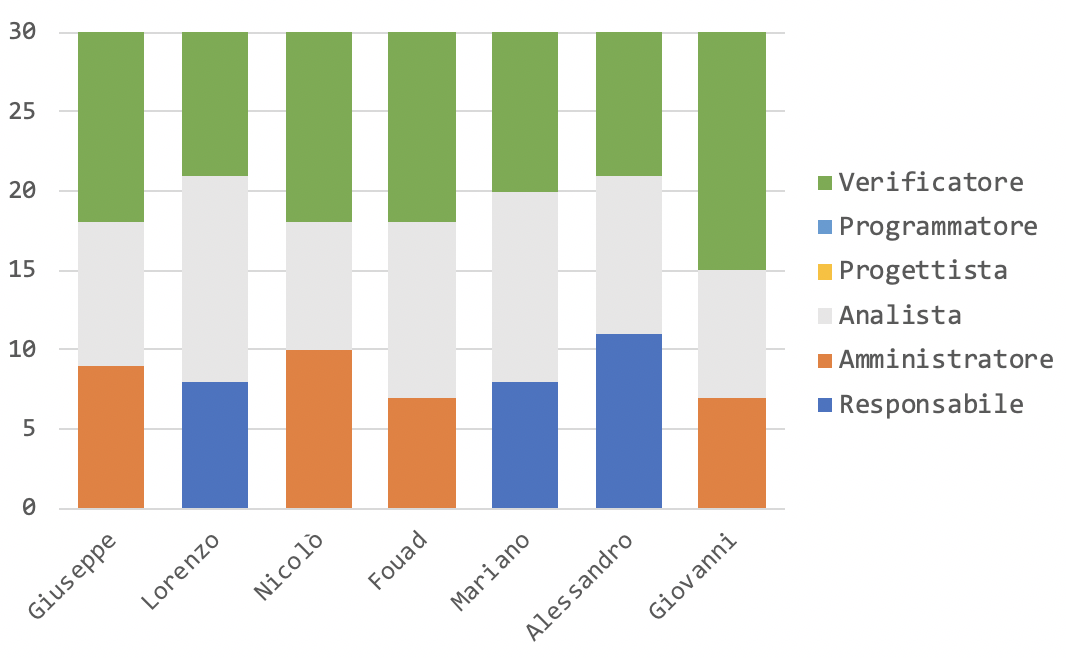
\includegraphics[width=0.8\linewidth]{./images/preventivo/analisi1.png}
				\caption{Grafico ore/ruolo componenti nella fase di analisi dei requisiti}
				\label{fig:grafico suddivione ruoli fase analisi dei requisiti}
			\end{figure}
		
			\subsubsection{Prospetto economico}
			In base al prospetto orario, quello economico sarà il seguente: 
			
			\rowcolors{2}{white}{lightest-grayest}
			\begin{longtable}{|c|c|c|c|c|c|c|c|}
				\hline
				\rowcolor{lighter-grayer}
				\textbf{Ruolo} & \textbf{Ore} & \textbf{Costo in €} \\
				\hline
				\endfirsthead
				
				\hline
				Responsabile & 27 & 810,00\\
				\hline
				\hline
				Amministratore & 33 & 660,00\\
				\hline
				\hline
				Analista & 71 & 1.775,00\\
				\hline
				\hline
				Progettista & - & -\\
				\hline
				\hline
				Programmatore & - & -\\
				\hline
				\hline
				Verificatore & 79 & 1.185,00\\
				\hline
				\textbf{Totale} & 210 & 4.430,00\\
				\hline
				\caption{Tabella contenente il prospetto economico in riferimento al prospetto orario nella tabella 4}
			\end{longtable}
			\pagebreak
		
			La tabella può essere riassunta nel seguente areogramma:
			\begin{figure}[H]
				\centering
				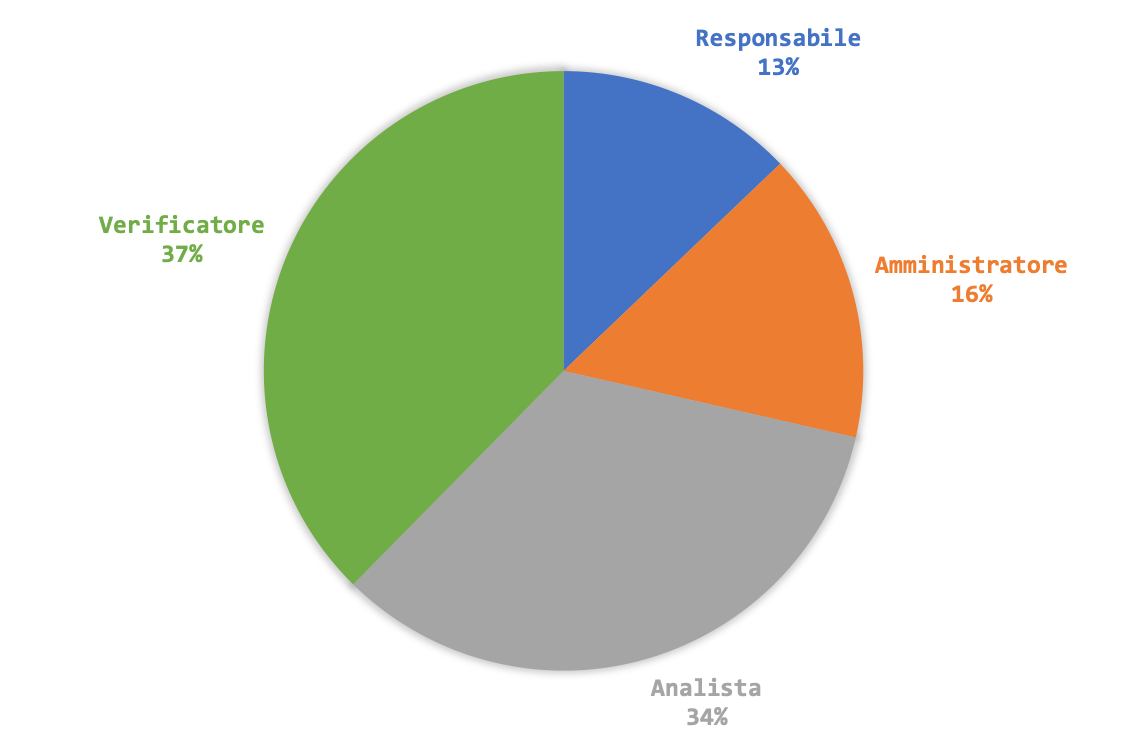
\includegraphics[width=0.8\linewidth]{./images/preventivo/analisi2.png}
				\caption{Grafico percentuale ore/ruolo nella fase di analisi dei requisiti}
				\label{fig:grafico costi ruolo fase analisi dei requisiti}
			\end{figure}
		
		
		
	\subsection{Fase di consolidamento dei requisiti}
			\subsubsection{Prospetto orario}
			Durante la fase di consolidamento dei requisiti la distribuzione oraria preventivata dei ruoli di ogni componente del gruppo sarà la seguente:
			
			\rowcolors{2}{lightest-grayest}{white}
			\begin{longtable}{|c|c|c|c|c|c|c|c|}
				\hline
				\rowcolor{lighter-grayer}
				\textbf{Nome} & \textbf{Re} & \textbf{Am} & \textbf{An} & \textbf{Pg}  & \textbf{Pr}   & \textbf{Ve} & \textbf{Totale} \\
				\hline
				\endfirsthead
				
				\hline
				Giuseppe Vito Bitetti & 0 & 0 & 5 & 0 & 0 & 0 & 5\\
				\hline
				\hline
				Lorenzo Dei Negri & 0 & 5 & 0 & 0 & 0 & 0 & 5\\
				\hline
				\hline
				Nicolò Frison & 0 & 0 & 0 & 0 & 0 & 5 & 5\\
				\hline
				\hline
				Fouad Mouad & 2 & 0 & 0 & 0 & 0 & 3 & 5\\
				\hline
				\hline
				Mariano Sciacco & 0 & 0 & 3 & 0 & 0 & 2 & 5\\
				\hline
				\hline
				Alessandro Tommasin & 0 & 0 & 4 & 0 & 0 & 1 & 5\\
				\hline
				\hline
				Giovanni Vidotto & 2 & 0 & 0 & 0 & 0 & 3 & 5\\
				\hline 
				\textbf{Totale} & 4 &  5 & 12 & 0 & 0 & 14 & 35\\
				\hline
				\caption{Tabella contenente la distribuzione oraria preventivata per il periodo di consolidamento dei requisiti}
			\end{longtable}
			\pagebreak
		
			La tabella può essere riassunta nel seguente istogramma:
			\begin{figure}[H]
				\centering
				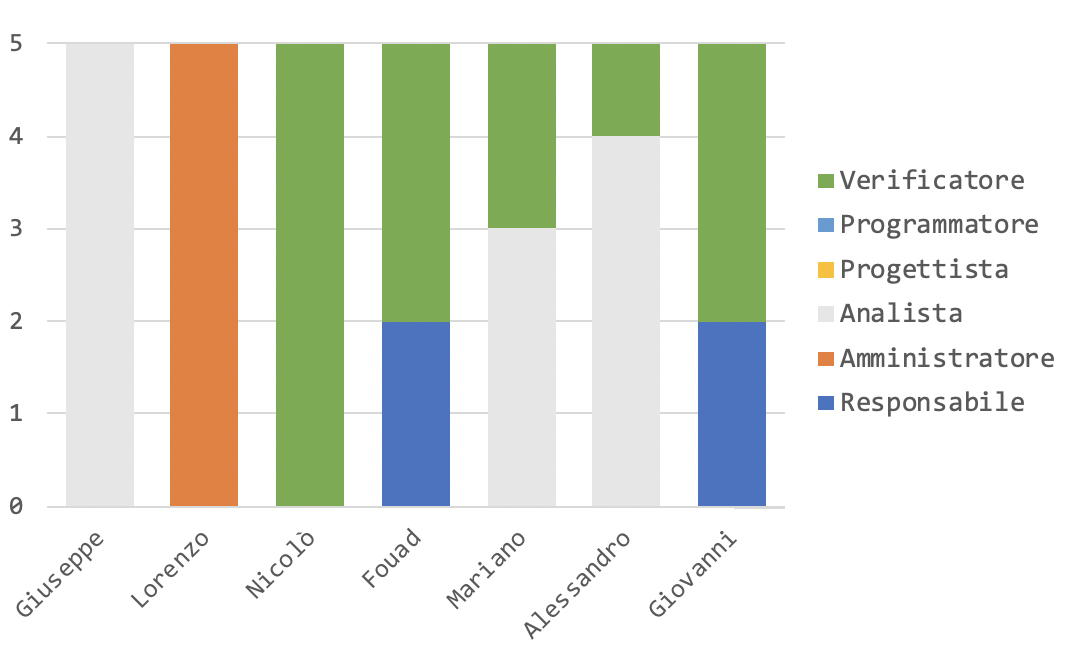
\includegraphics[width=0.8\linewidth]{./images/preventivo/consRequisiti1.png}
				\caption{Grafico ore/ruolo componenti nella fase di consolidamento dei requisiti}
				\label{fig:grafico suddivione ruoli fase consolidamento requisiti}
			\end{figure}
		
		\subsubsection{Prospetto economico}
		In base al prospetto orario, quello economico sarà il seguente: 
		
			\rowcolors{2}{white}{lightest-grayest}
			\begin{longtable}{|c|c|c|c|c|c|c|c|}
				\hline
				\rowcolor{lighter-grayer}
				\textbf{Ruolo} & \textbf{Ore} & \textbf{Costo in €} \\
				\hline
				\endfirsthead
				
				\hline
				Responsabile & 4 & 120,00\\
				\hline
				\hline
				Amministratore & 5 & 100,00\\
				\hline
				\hline
				Analista & 12 & 300,00\\
				\hline
				\hline
				Progettista & - & -\\
				\hline
				\hline
				Programmatore & -  & -\\
				\hline
				\hline
				Verificatore & 14 & 210,00\\
				\hline
				\textbf{Totale} & 35 & 730,00\\
				\hline
				\caption{Tabella contenente il prospetto economico in riferimento al prospetto orario nella tabella 6}
			\end{longtable}
			\pagebreak
			
			La tabella può essere riassunta nel seguente areogramma:
			\begin{figure}[H]
				\centering
				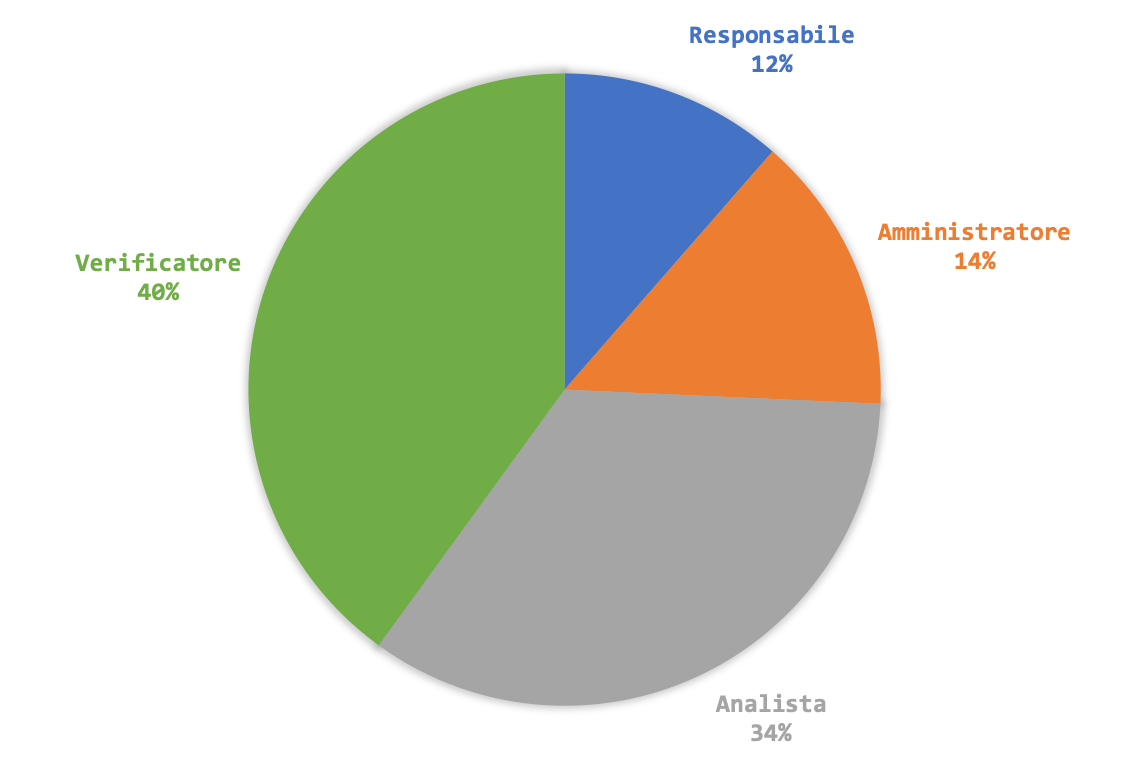
\includegraphics[width=0.8\linewidth]{./images/preventivo/consRequisiti2.png}
				\caption{Grafico percentuale ore/ruolo nella fase di consolidamento dei requisiti}
				\label{fig:grafico costi ruolo fase consolidamento dei requisiti}
			\end{figure}
	
	
	
	\subsection{Fase di progettazione della technology baseline e correzioni documenti}
		\subsubsection{Prospetto orario}
		Durante questa fase verranno stabiliti gli incrementi, corretti i documenti e progettata la \textit{technology baseline}. La distribuzione oraria preventivata dei ruoli di ogni componente del gruppo sarà la seguente:
		
		\rowcolors{2}{lightest-grayest}{white}
		\begin{longtable}{|c|c|c|c|c|c|c|c|}
			\hline
			\rowcolor{lighter-grayer}
			\textbf{Nome} & \textbf{Re} & \textbf{Am} & \textbf{An} & \textbf{Pg}  & \textbf{Pr}   & \textbf{Ve} & \textbf{Totale} \\
			\hline
			\endfirsthead
			
			\hline
			Giuseppe Vito Bitetti 		& 3 & 0 & 7 & 0 & 0 & 3 & 13\\
			\hline
			\hline
			Lorenzo Dei Negri			& 0 & 5 & 1 & 5 & 0 & 2 & 13\\
			\hline
			\hline
			Nicolò Frison				   & 0 & 3 & 5 & 5 & 0 & 0 & 13\\
			\hline
			\hline
			Fouad Mouad 				& 0 & 4 & 3 & 2 & 0 & 4 & 13\\
			\hline
			\hline
			Mariano Sciacco 			& 3& 0 & 1 & 9 & 0 & 0 & 13\\
			\hline
			\hline
			Alessandro Tommasin    & 0 & 4 & 6 & 0 & 0 & 3 & 13\\
			\hline
			\hline
			Giovanni Vidotto 			& 2 & 0 & 5 & 2 & 0 & 4 & 13\\
			\hline 
			\textbf{Totale}			 & 8 &  16 & 28 & 23 & 0 & 16 & 91\\
			\hline
			\caption{Tabella contenente il prospetto orario preventivato per il periodo di progettazione della technology baseline}
		\end{longtable}
		\pagebreak
		
		La tabella può essere riassunta nel seguente istogramma:
		\begin{figure}[H]
			\centering
			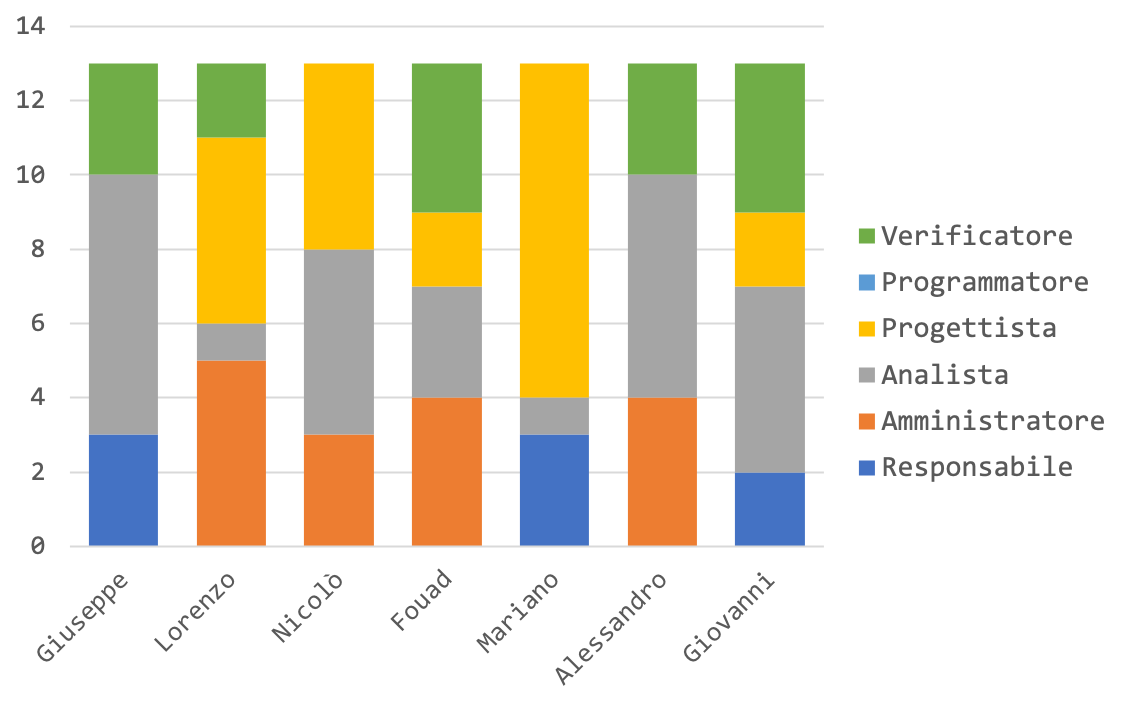
\includegraphics[width=0.8\linewidth]{./images/preventivo/progArch1.png}
			\caption{Grafico ore/ruolo componenti nella fase di progettazione della technology baseline}
			\label{fig:grafico suddivione ruoli fase progettazione della technology baseline}
		\end{figure}
	
		\subsubsection{Prospetto economico}
		In base al prospetto orario, quello economico sarà il seguente: 
		
		\rowcolors{2}{white}{lightest-grayest}
		\begin{longtable}{|c|c|c|c|c|c|c|c|}
			\hline
			\rowcolor{lighter-grayer}
			\textbf{Ruolo} & \textbf{Ore} & \textbf{Costo in € } \\
			\hline
			\endfirsthead
			
			\hline
			Responsabile 	    & 8 & 240,00\\
			\hline 
			\hline
			Amministratore	  & 16 & 320,00\\
			\hline
			\hline
			Analista 				& 28 & 700,00\\
			\hline
			\hline
			Progettista 		  & 23 & 506,00\\
			\hline
			\hline
			Programmatore 	 & 0 & 0,00\\
			\hline
			\hline
			Verificatore 		  & 16 & 240,00\\
			\hline
			\textbf{Totale} 	& 91 & 2.0006,00\\
			\hline
			\caption{Tabella contenente il prospetto economico in riferimento al prospetto orario nella tabella 8}
		\end{longtable}
		\pagebreak
		
		La tabella può essere riassunta nel seguente areogramma:
		\begin{figure}[H]
			\centering
			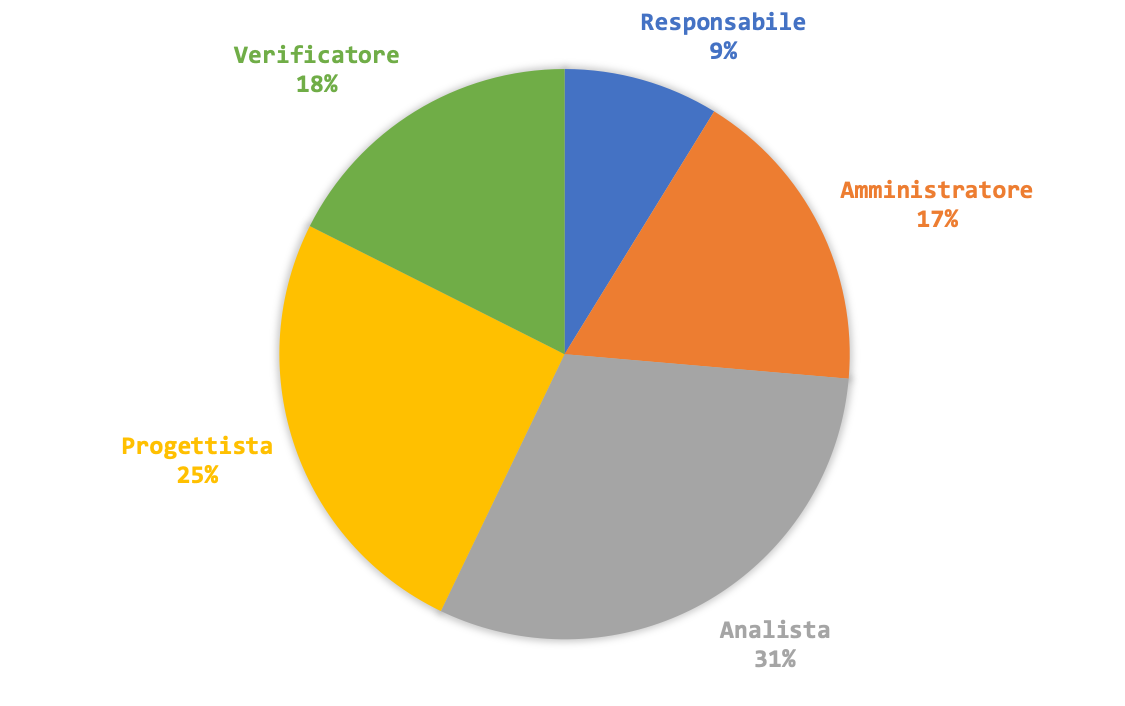
\includegraphics[width=0.8\linewidth]{./images/preventivo/progArch2.png}
			\caption{Grafico percentuale ore/ruolo nella fase di progettazione della technology baseline}
			\label{fig:grafico costi ruolo fase progettazione della technology baseline}
		\end{figure}
	
	
	\subsection{Incremento I}
		\subsubsection{Prospetto orario}
		Durante il primo incremento la distribuzione oraria preventivata dei ruoli di ogni componente del gruppo sarà la seguente:
		
		\rowcolors{2}{lightest-grayest}{white}
		\begin{longtable}{|c|c|c|c|c|c|c|c|}
			\hline
			\rowcolor{lighter-grayer}
			\textbf{Nome} & \textbf{Re} & \textbf{Am} & \textbf{An} & \textbf{Pg}  & \textbf{Pr}   & \textbf{Ve} & \textbf{Totale} \\
			\hline
			\endfirsthead
			
			\hline
			Giuseppe Vito Bitetti 		 & 0 & 0 & 3 & 0 & 2 & 0 & 5\\
			\hline
			\hline
			Lorenzo Dei Negri			 & 0 & 0 & 0 & 2 & 0 & 3 & 5\\
			\hline
			\hline
			Nicolò Frison				    & 0 & 3 & 0 & 0 & 0 & 2 & 5\\
			\hline
			\hline
			Fouad Mouad 				 & 3 & 0 & 2 & 0 & 0 & 0 & 5\\
			\hline
			\hline
			Mariano Sciacco 			 & 0 & 0 & 0 & 3 & 2 & 0 & 5\\
			\hline
			\hline
			Alessandro Tommasin     & 6 & 2 & 0 & 3 & 0 & 0 & 5\\
			\hline
			\hline
			Giovanni Vidotto 			 & 0 & 0 & 0 & 8 & 4 & 1 & 5\\
			\hline 
			\textbf{Totale}			 		& 3 & 5 & 5 & 8 & 8 & 6 & 35\\
			\hline
			\caption{Tabella contenente il prospetto orario preventivato per il primo incremento}
		\end{longtable}
		\pagebreak
		
		La tabella può essere riassunta nel seguente istogramma:
		\begin{figure}[H]
			\centering
			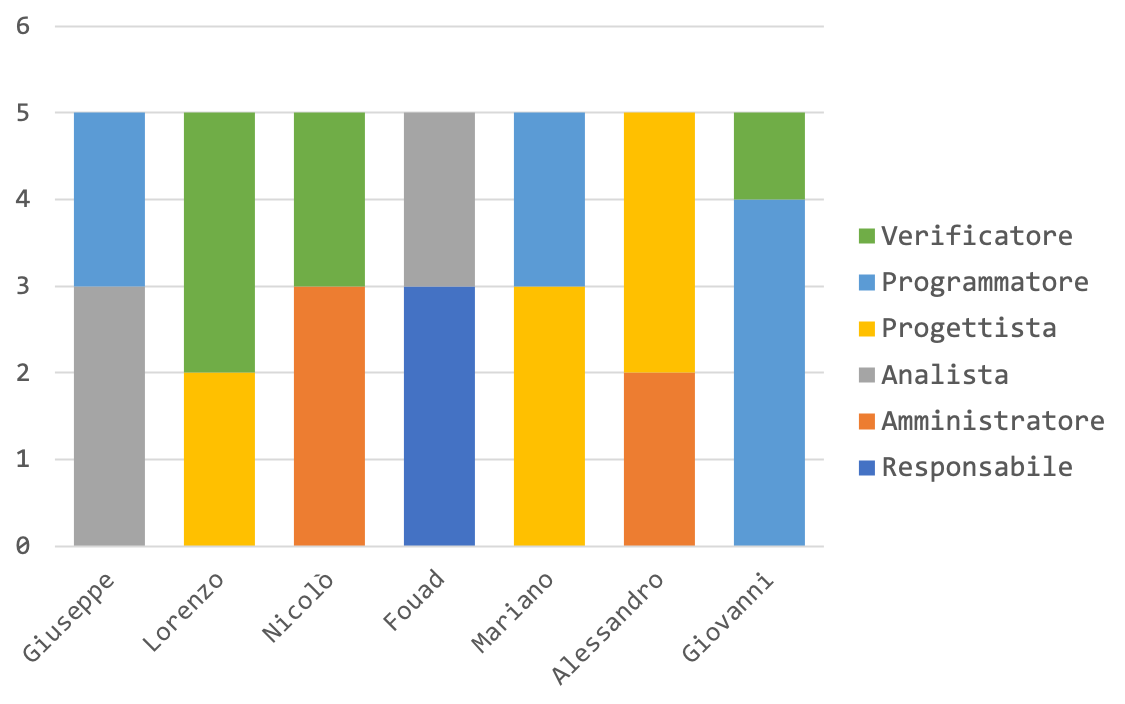
\includegraphics[width=0.8\linewidth]{./images/preventivo/incremento1-1.png}
			\caption{Grafico ore/ruolo componenti nel primo incremento}
			\label{fig:grafico suddivione ruoli incremento I}
		\end{figure}
	
		\subsubsection{Prospetto economico}
		In base al prospetto orario, quello economico sarà il seguente: 
		
		\rowcolors{2}{white}{lightest-grayest}
		\begin{longtable}{|c|c|c|c|c|c|c|c|}
			\hline
			\rowcolor{lighter-grayer}
			\textbf{Ruolo} & \textbf{Ore} & \textbf{Costo in € } \\
			\hline
			\endfirsthead
			
			\hline
			Responsabile 	    & 3 & 90,00\\
			\hline 
			\hline
			Amministratore	   & 5 & 100,00\\
			\hline
			\hline
			Analista 				& 5 & 125,00\\
			\hline
			\hline
			Progettista 		   & 8 & 176,00\\
			\hline
			\hline
			Programmatore 	  & 8 & 120,00\\
			\hline
			\hline
			Verificatore 		   & 6 & 90,00\\
			\hline
			\textbf{Totale} 	 & 35 & 701,00\\
			\hline
			\caption{Tabella contenente il prospetto economico in riferimento al prospetto orario nella tabella 10}
		\end{longtable}
		\pagebreak
		
		La tabella può essere riassunta nel seguente areogramma:
		\begin{figure}[H]
			\centering
			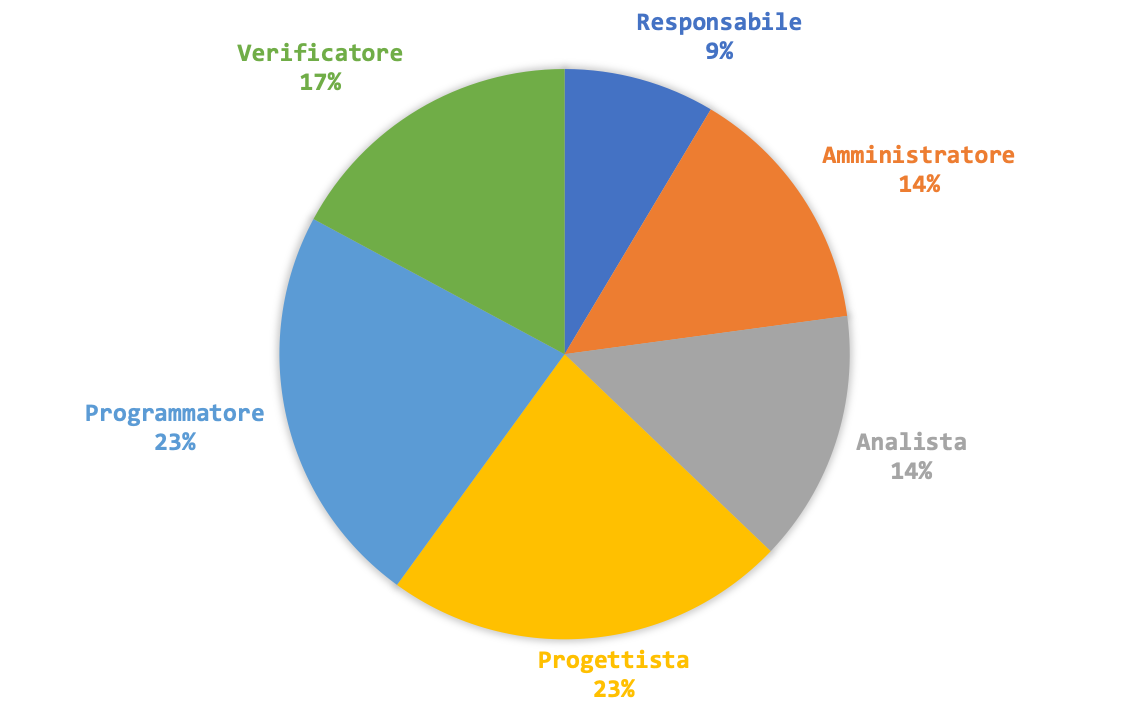
\includegraphics[width=0.8\linewidth]{./images/preventivo/incremento1-2.png}
			\caption{Grafico percentuale ore/ruolo del primo incremento}
			\label{fig:grafico costi ruolo incremento I}
		\end{figure}
	
	
	
	\subsection{Incremento II}
		\subsubsection{Prospetto orario}
		Durante il secondo incremento la distribuzione oraria preventivata dei ruoli di ogni componente del gruppo sarà la seguente:
		
		\rowcolors{2}{lightest-grayest}{white}
		\begin{longtable}{|c|c|c|c|c|c|c|c|}
			\hline
			\rowcolor{lighter-grayer}
			\textbf{Nome} & \textbf{Re} & \textbf{Am} & \textbf{An} & \textbf{Pg}  & \textbf{Pr}   & \textbf{Ve} & \textbf{Totale} \\
			\hline
			\endfirsthead
			
			\hline
			Giuseppe Vito Bitetti 		 & 0 & 0 & 0 & 3 & 0 & 3 & 6\\
			\hline
			\hline
			Lorenzo Dei Negri			 & 0 & 0 & 0 & 0 & 3 & 3 & 6\\
			\hline
			\hline
			Nicolò Frison				    & 2 & 0 & 0 & 0 & 4 & 0 & 6\\
			\hline
			\hline
			Fouad Mouad 				 & 0 & 4 & 2 & 0 & 0 & 0 & 6\\
			\hline
			\hline
			Mariano Sciacco 			 & 0 & 0 & 0 & 3 & 0 & 3 & 6\\
			\hline
			\hline
			Alessandro Tommasin     & 2 & 0 & 0 & 4 & 0 & 0 & 6\\
			\hline
			\hline
			Giovanni Vidotto 			 & 0 & 2 & 0 & 4 & 0 & 0 & 6\\
			\hline 
			\textbf{Totale}			 		& 4 & 6 & 2 & 8 & 8 & 6 & 42\\
			\hline
			\caption{Tabella contenente il prospetto orario preventivato per il secondo incremento}
		\end{longtable}
		\pagebreak
		
		La tabella può essere riassunta nel seguente istogramma:
		\begin{figure}[H]
			\centering
			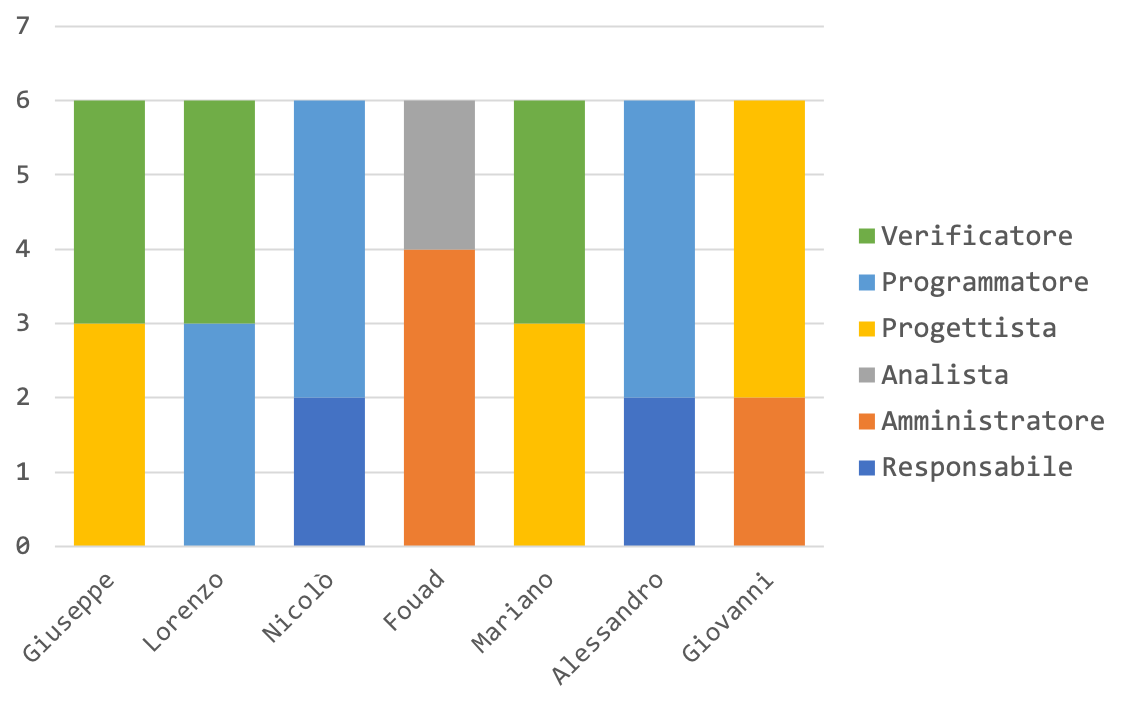
\includegraphics[width=0.8\linewidth]{./images/preventivo/incremento2-1.png}
			\caption{Grafico ore/ruolo componenti secondo incremento}
			\label{fig:grafico suddivione ruoli incremento II}
		\end{figure}
		
		\subsubsection{Prospetto economico}
		In base al prospetto orario, quello economico sarà il seguente: 
		
		\rowcolors{2}{white}{lightest-grayest}
		\begin{longtable}{|c|c|c|c|c|c|c|c|}
			\hline
			\rowcolor{lighter-grayer}
			\textbf{Ruolo} & \textbf{Ore} & \textbf{Costo in € } \\
			\hline
			\endfirsthead
			
			\hline
			Responsabile 	    & 4 & 120,00\\
			\hline 
			\hline
			Amministratore	   & 6 & 120,00\\
			\hline
			\hline
			Analista 				& 2 & 50,00\\
			\hline
			\hline
			Progettista 		   & 10 & 220,00\\
			\hline
			\hline
			Programmatore 	  & 11 & 165,00\\
			\hline
			\hline
			Verificatore 		   & 9 & 135,00\\
			\hline
			\textbf{Totale} 	 & 42 & 810,00\\
			\hline
			\caption{Tabella contenente il prospetto economico in riferimento al prospetto orario nella tabella 10}
		\end{longtable}
		\pagebreak
		
		La tabella può essere riassunta nel seguente areogramma:
		\begin{figure}[H]
			\centering
			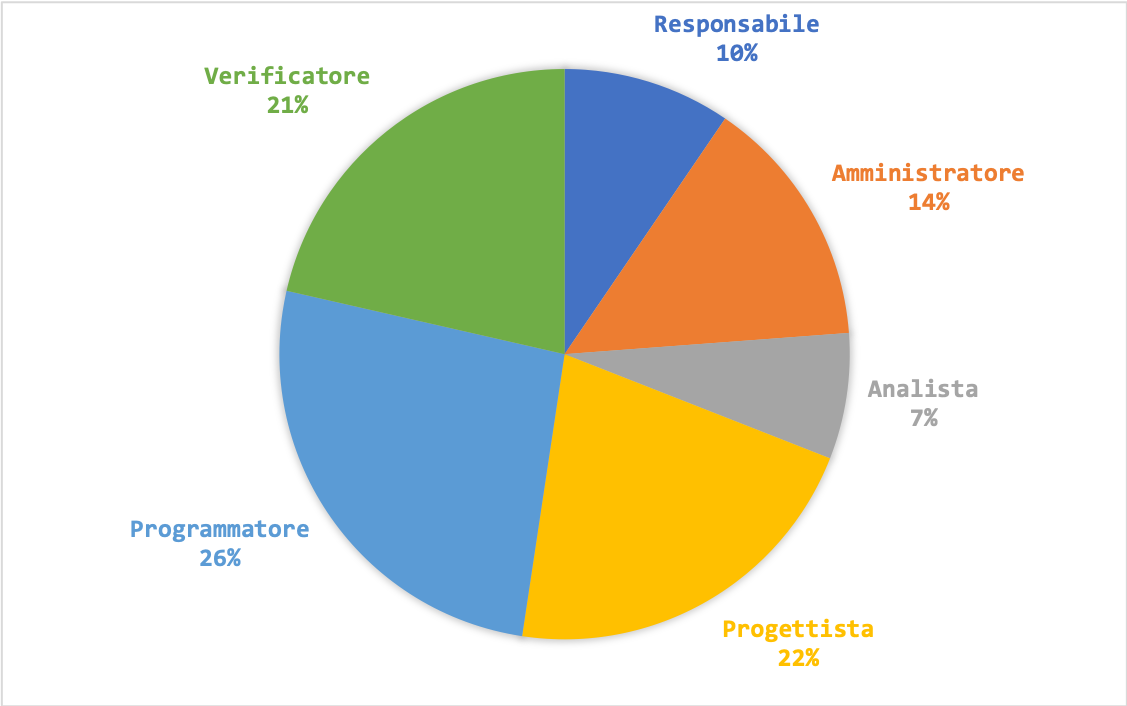
\includegraphics[width=0.8\linewidth]{./images/preventivo/incremento2-2.png}
			\caption{Grafico percentuale ore/ruolo del secondo incremento}
			\label{fig:grafico costi ruolo incremento II}
		\end{figure}


		
	\subsection{Incremento III}
		\subsubsection{Prospetto orario}
		Durante il terzo incremento la distribuzione oraria preventivata dei ruoli di ogni componente del gruppo sarà la seguente:
		
		\rowcolors{2}{lightest-grayest}{white}
		\begin{longtable}{|c|c|c|c|c|c|c|c|}
			\hline
			\rowcolor{lighter-grayer}
			\textbf{Nome} & \textbf{Re} & \textbf{Am} & \textbf{An} & \textbf{Pg}  & \textbf{Pr}   & \textbf{Ve} & \textbf{Totale} \\
			\hline
			\endfirsthead
			
			\hline
			Giuseppe Vito Bitetti 		 & 0 & 0 & 0 & 0 & 3 & 3 & 6\\
			\hline
			\hline
			Lorenzo Dei Negri			 & 0 & 0 & 0 & 3 & 0 & 3 & 6\\
			\hline
			\hline
			Nicolò Frison				    & 1 & 0 & 0 & 2 & 0 & 3 & 6\\
			\hline
			\hline
			Fouad Mouad 				 & 0 & 0 & 0 & 3 & 3 & 0 & 6\\
			\hline
			\hline
			Mariano Sciacco 			 & 0 & 3 & 0 & 0 & 3 & 0 & 6\\
			\hline
			\hline
			Alessandro Tommasin     & 2 & 0 & 0 & 2 & 2 & 0 & 6\\
			\hline
			\hline
			Giovanni Vidotto 			 & 0 & 0 & 0 & 2 & 0 & 4 & 6\\
			\hline 
			\textbf{Totale}			 		& 3 & 3 & 0 & 12 & 11 & 13 & 42\\
			\hline
			\caption{Tabella contenente il prospetto orario preventivato per terzo incremento}
		\end{longtable}
		\pagebreak
		
		La tabella può essere riassunta nel seguente istogramma:
		\begin{figure}[H]
			\centering
			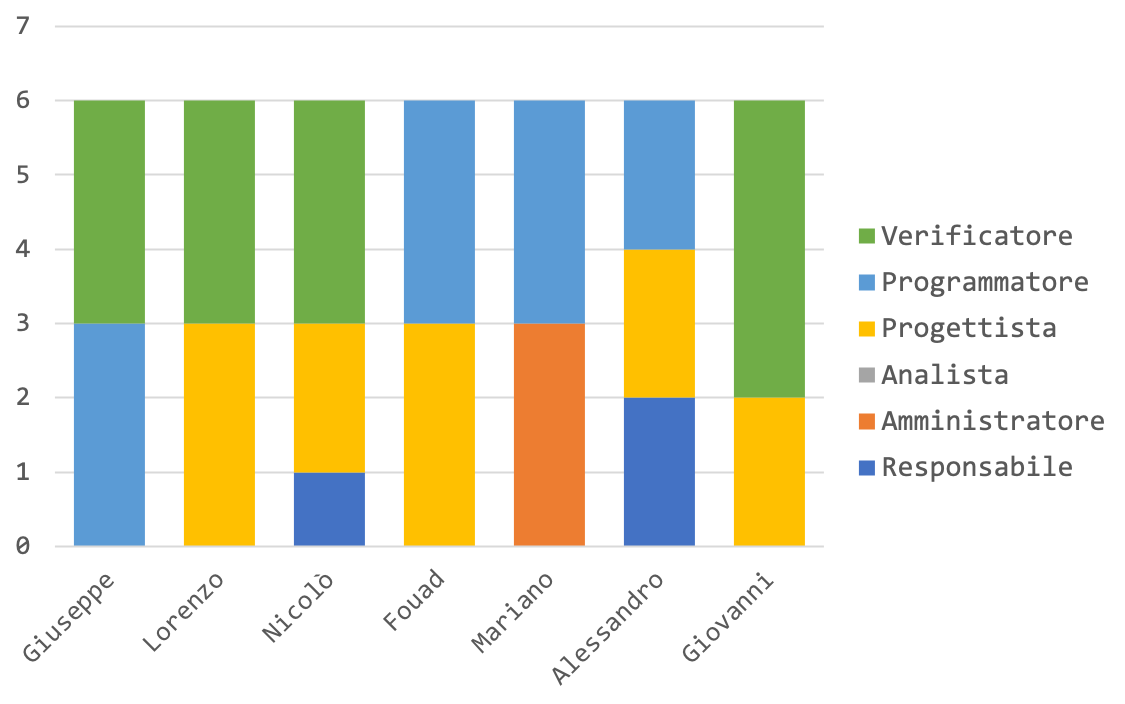
\includegraphics[width=0.8\linewidth]{./images/preventivo/incremento3-1.png}
			\caption{Grafico ore/ruolo componenti terzo incremento}
			\label{fig:grafico suddivione ruoli incremento III}
		\end{figure}
		
		\subsubsection{Prospetto economico}
		In base al prospetto orario, quello economico sarà il seguente: 
		
		\rowcolors{2}{white}{lightest-grayest}
		\begin{longtable}{|c|c|c|c|c|c|c|c|}
			\hline
			\rowcolor{lighter-grayer}
			\textbf{Ruolo} & \textbf{Ore} & \textbf{Costo in € } \\
			\hline
			\endfirsthead
			
			\hline
			Responsabile 	    & 3 & 90,00\\
			\hline 
			\hline
			Amministratore	   & 3 & 60,00\\
			\hline
			\hline
			Analista 				& 0 & 0,00\\
			\hline
			\hline
			Progettista 		   & 12 & 264,00\\
			\hline
			\hline
			Programmatore 	  & 11 & 165,00\\
			\hline
			\hline
			Verificatore 		   & 13 & 195,00\\
			\hline
			\textbf{Totale} 	 & 42 & 774,00\\
			\hline
			\caption{Tabella contenente il prospetto economico in riferimento al prospetto orario}
		\end{longtable}
		\pagebreak
		
		La tabella può essere riassunta nel seguente areogramma:
		\begin{figure}[H]
			\centering
			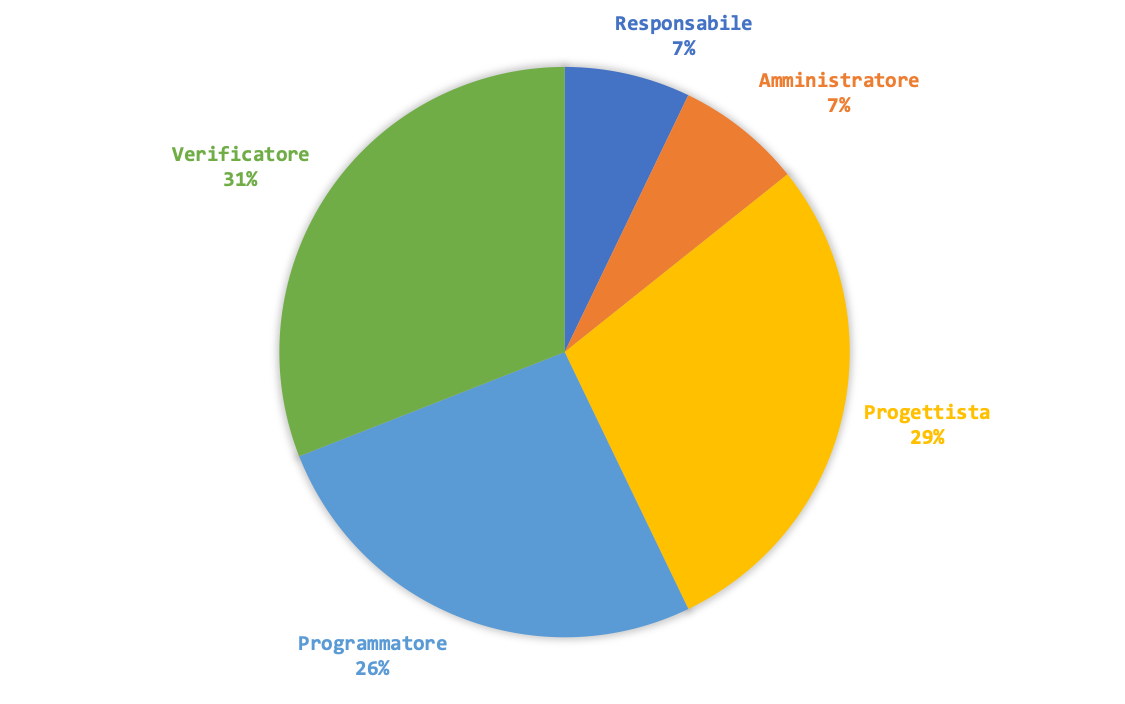
\includegraphics[width=0.8\linewidth]{./images/preventivo/incremento3-2.png}
			\caption{Grafico percentuale ore/ruolo terzo incremento}
			\label{fig:grafico costi ruolo incremento III}
		\end{figure}
		
		
		
	\subsection{Incremento IV}
		\subsubsection{Prospetto orario}
		Durante il quarto incremento la distribuzione oraria preventivata dei ruoli di ogni componente del gruppo sarà la seguente:
		
		\rowcolors{2}{lightest-grayest}{white}
		\begin{longtable}{|c|c|c|c|c|c|c|c|}
			\hline
			\rowcolor{lighter-grayer}
			\textbf{Nome} & \textbf{Re} & \textbf{Am} & \textbf{An} & \textbf{Pg}  & \textbf{Pr}   & \textbf{Ve} & \textbf{Totale} \\
			\hline
			\endfirsthead
			
			\hline
			Giuseppe Vito Bitetti 		 & 2 & 0 & 0 & 0 & 4 & 0 & 6\\
			\hline
			\hline
			Lorenzo Dei Negri			 & 2 & 0 & 2 & 2 & 0 & 0 & 6\\
			\hline
			\hline
			Nicolò Frison				    & 0 & 0 & 0 & 2 & 4 & 0 & 6\\
			\hline
			\hline
			Fouad Mouad 				 & 0 & 3 & 0 & 0 & 0 & 3 & 6\\
			\hline
			\hline
			Mariano Sciacco 			 & 3 & 0 & 0 & 0 & 3 & 0 & 6\\
			\hline
			\hline
			Alessandro Tommasin     & 0 & 0 & 2 & 0 & 0 & 4 & 6\\
			\hline
			\hline
			Giovanni Vidotto 			 & 0 & 0 & 0 & 5 & 0 & 1 & 6\\
			\hline 
			\textbf{Totale}			 		& 7 & 3 & 4 & 9 & 11 & 8 & 42\\
			\hline
			\caption{Tabella contenente il prospetto orario preventivato per quarto incremento}
		\end{longtable}
		\pagebreak
		
		La tabella può essere riassunta nel seguente istogramma:
		\begin{figure}[H]
			\centering
			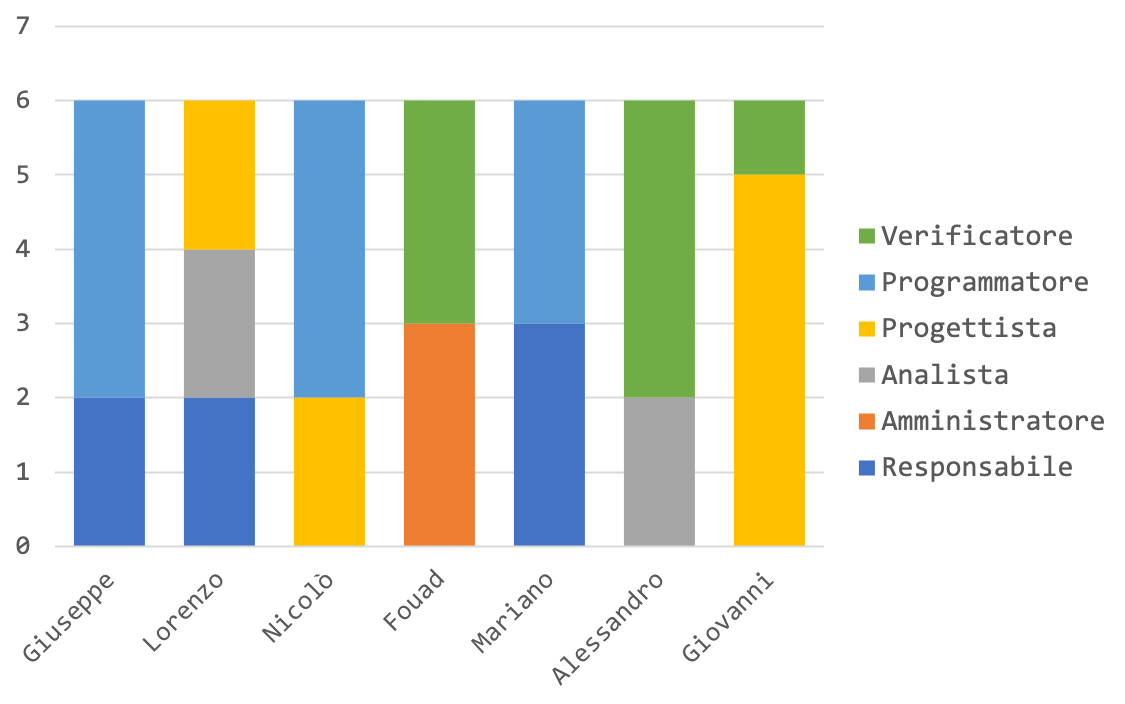
\includegraphics[width=0.8\linewidth]{./images/preventivo/incremento4-1.png}
			\caption{Grafico ore/ruolo componenti quarto  incremento}
			\label{fig:grafico suddivione ruoli incremento IV}
		\end{figure}
		
		\subsubsection{Prospetto economico}
		In base al prospetto orario, quello economico sarà il seguente: 
		
		\rowcolors{2}{white}{lightest-grayest}
		\begin{longtable}{|c|c|c|c|c|c|c|c|}
			\hline
			\rowcolor{lighter-grayer}
			\textbf{Ruolo} & \textbf{Ore} & \textbf{Costo in € } \\
			\hline
			\endfirsthead
			
			\hline
			Responsabile 	    & 7 & 210,00\\
			\hline 
			\hline
			Amministratore	   & 3 & 60,00\\
			\hline
			\hline
			Analista 				& 4 & 100,00\\
			\hline
			\hline
			Progettista 		   & 9 & 198,00\\
			\hline
			\hline
			Programmatore 	  & 11 & 165,00\\
			\hline
			\hline
			Verificatore 		   & 8 & 120,00\\
			\hline
			\textbf{Totale} 	 & 42 & 853,00\\
			\hline
			\caption{Tabella contenente il prospetto economico in riferimento al prospetto orario }
		\end{longtable}
		\pagebreak
		
		La tabella può essere riassunta nel seguente areogramma:
		\begin{figure}[H]
			\centering
			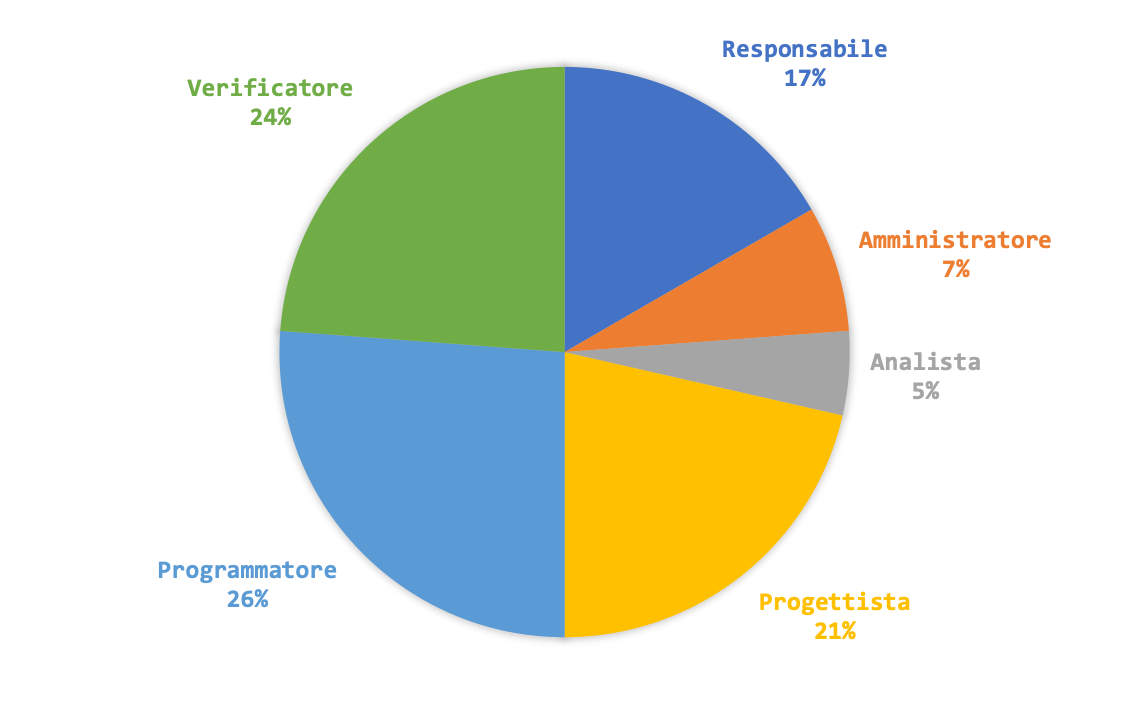
\includegraphics[width=0.8\linewidth]{./images/preventivo/incremento4-2.png}
			\caption{Grafico percentuale ore/ruolo quarto incremento}
			\label{fig:grafico costi ruolo incremento IV}
		\end{figure}
		
		
		
	\subsection{Incremento V}
		\subsubsection{Prospetto orario}
		Durante il quinto incremento la distribuzione oraria preventivata dei ruoli di ogni componente del gruppo sarà la seguente:
		
		\rowcolors{2}{lightest-grayest}{white}
		\begin{longtable}{|c|c|c|c|c|c|c|c|}
			\hline
			\rowcolor{lighter-grayer}
			\textbf{Nome} & \textbf{Re} & \textbf{Am} & \textbf{An} & \textbf{Pg}  & \textbf{Pr}   & \textbf{Ve} & \textbf{Totale} \\
			\hline
			\endfirsthead
			
			\hline
			Giuseppe Vito Bitetti 		 & 0 & 2 & 2 & 0 & 0 & 2 & 6\\
			\hline
			\hline
			Lorenzo Dei Negri			 & 0 & 0 & 0 & 2 & 4 & 0 & 6\\
			\hline
			\hline
			Nicolò Frison				    & 2 & 0 & 0 & 0 & 0 & 4 & 6\\
			\hline
			\hline
			Fouad Mouad 				 & 2 & 0 & 0 & 0 & 4 & 0 & 6\\
			\hline
			\hline
			Mariano Sciacco 			 & 0 & 0 & 0 & 1 & 3 & 2 & 6\\
			\hline
			\hline
			Alessandro Tommasin     & 0 & 0 & 0 & 3 & 3 & 0 & 6\\
			\hline
			\hline
			Giovanni Vidotto 			 & 0 & 2 & 0 & 0 & 4 & 0 & 6\\
			\hline 
			\textbf{Totale}			 		& 4 & 4 & 2 & 6 & 18 & 8 & 42\\
			\hline
			\caption{Tabella contenente il prospetto orario preventivato per il quinto incremento}
		\end{longtable}
		\pagebreak
		
		La tabella può essere riassunta nel seguente istogramma:
		\begin{figure}[H]
			\centering
			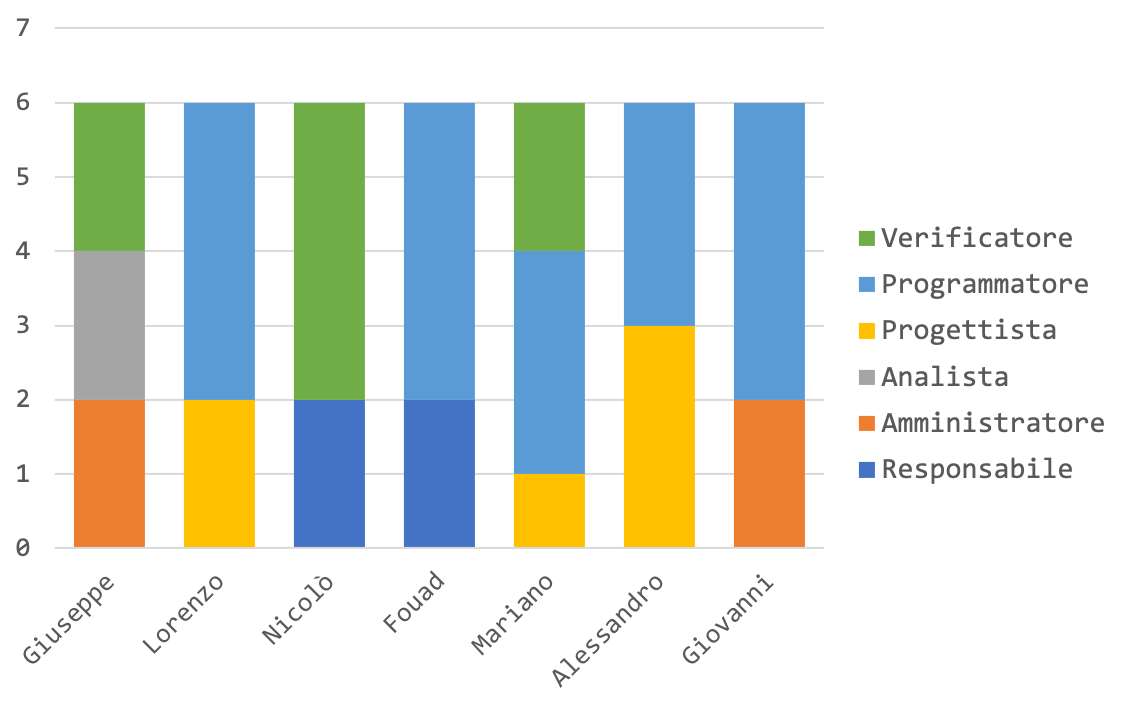
\includegraphics[width=0.8\linewidth]{./images/preventivo/incremento5-1.png}
			\caption{Grafico ore/ruolo componenti quinto incremento}
			\label{fig:grafico suddivione ruoli incremento V}
		\end{figure}
		
		\subsubsection{Prospetto economico}
		In base al prospetto orario, quello economico sarà il seguente: 
		
		\rowcolors{2}{white}{lightest-grayest}
		\begin{longtable}{|c|c|c|c|c|c|c|c|}
			\hline
			\rowcolor{lighter-grayer}
			\textbf{Ruolo} & \textbf{Ore} & \textbf{Costo in € } \\
			\hline
			\endfirsthead
			
			\hline
			Responsabile 	    & 3 & 90,00\\
			\hline 
			\hline
			Amministratore	   & 3 & 60,00\\
			\hline
			\hline
			Analista 				& 0 & 0,00\\
			\hline
			\hline
			Progettista 		   & 12 & 264,00\\
			\hline
			\hline
			Programmatore 	  & 11 & 165,00\\
			\hline
			\hline
			Verificatore 		   & 13 & 195,00\\
			\hline
			\textbf{Totale} 	 & 42 & 774,00\\
			\hline
			\caption{Tabella contenente il prospetto economico in riferimento al prospetto orario}
		\end{longtable}
		\pagebreak
		
		La tabella può essere riassunta nel seguente areogramma:
		\begin{figure}[H]
			\centering
			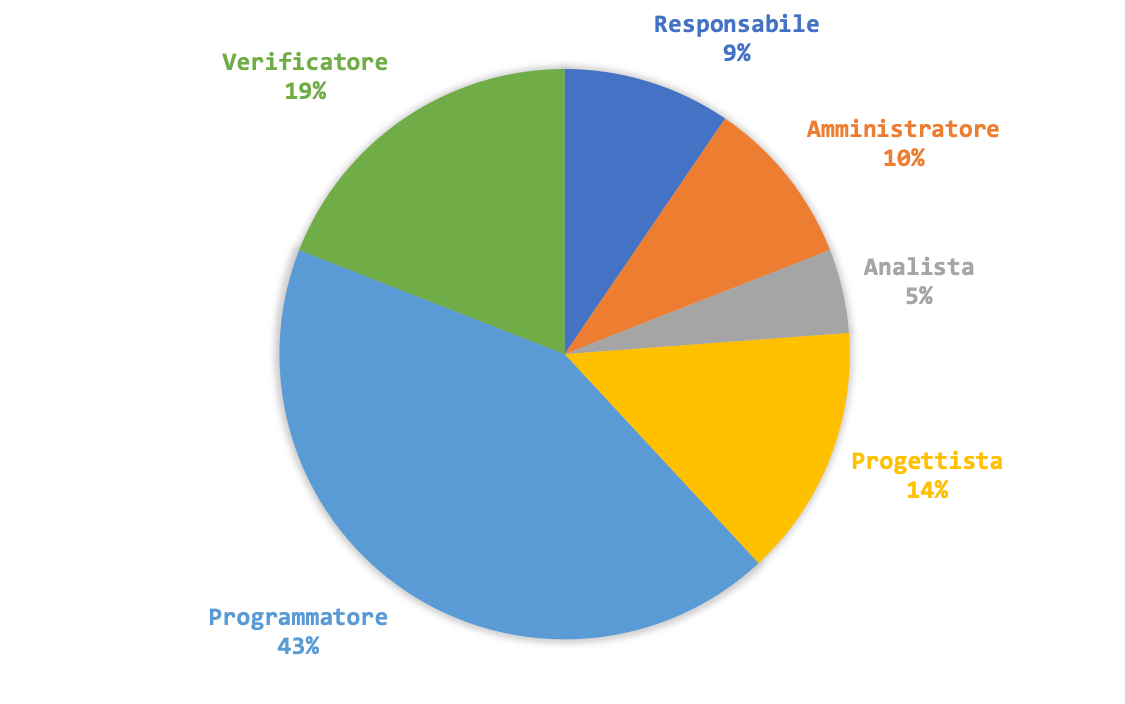
\includegraphics[width=0.8\linewidth]{./images/preventivo/incremento5-2.png}
			\caption{Grafico percentuale ore/ruolo quinto incremento}
			\label{fig:grafico costi ruolo incremento V}
		\end{figure}
		
		
		
	\subsection{Incremento VI}
		\subsubsection{Prospetto orario}
		Durante il sesto incremento la distribuzione oraria preventivata dei ruoli di ogni componente del gruppo sarà la seguente:
		
		\rowcolors{2}{lightest-grayest}{white}
		\begin{longtable}{|c|c|c|c|c|c|c|c|}
			\hline
			\rowcolor{lighter-grayer}
			\textbf{Nome} & \textbf{Re} & \textbf{Am} & \textbf{An} & \textbf{Pg}  & \textbf{Pr}   & \textbf{Ve} & \textbf{Totale} \\
			\hline
			\endfirsthead
			
			\hline
			Giuseppe Vito Bitetti 		 & 0 & 0 & 0 & 0 & 3 & 3 & 6\\
			\hline
			\hline
			Lorenzo Dei Negri			 & 0 & 0 & 0 & 3 & 0 & 3 & 6\\
			\hline
			\hline
			Nicolò Frison				    & 1 & 0 & 0 & 2 & 0 & 3 & 6\\
			\hline
			\hline
			Fouad Mouad 				 & 0 & 0 & 0 & 3 & 3 & 0 & 6\\
			\hline
			\hline
			Mariano Sciacco 			 & 0 & 3 & 0 & 0 & 3 & 0 & 6\\
			\hline
			\hline
			Alessandro Tommasin     & 2 & 0 & 0 & 2 & 2 & 0 & 6\\
			\hline
			\hline
			Giovanni Vidotto 			 & 0 & 0 & 0 & 2 & 0 & 4 & 6\\
			\hline 
			\textbf{Totale}			 		& 3 & 3 & 0 & 12 & 11 & 13 & 42\\
			\hline
			\caption{Tabella contenente il prospetto orario preventivato per il sesto incremento}
		\end{longtable}
		\pagebreak
		
		La tabella può essere riassunta nel seguente istogramma:
		\begin{figure}[H]
			\centering
			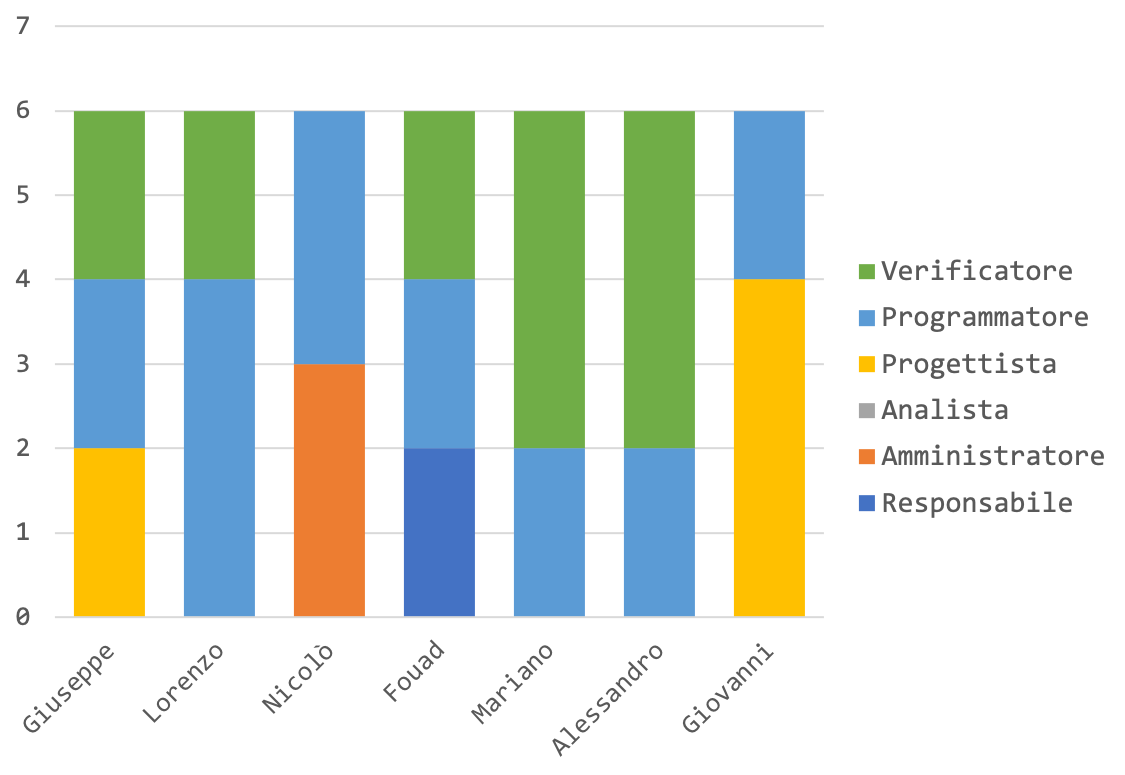
\includegraphics[width=0.8\linewidth]{./images/preventivo/incremento6-1.png}
			\caption{Grafico ore/ruolo componenti sesto incremento}
			\label{fig:grafico suddivione ruoli incremento VI}
		\end{figure}
		
		\subsubsection{Prospetto economico}
		In base al prospetto orario, quello economico sarà il seguente: 
		
		\rowcolors{2}{white}{lightest-grayest}
		\begin{longtable}{|c|c|c|c|c|c|c|c|}
			\hline
			\rowcolor{lighter-grayer}
			\textbf{Ruolo} & \textbf{Ore} & \textbf{Costo in € } \\
			\hline
			\endfirsthead
			
			\hline
			Responsabile 	    & 3 & 90,00\\
			\hline 
			\hline
			Amministratore	   & 3 & 60,00\\
			\hline
			\hline
			Analista 				& 0 & 0,00\\
			\hline
			\hline
			Progettista 		   & 12 & 264,00\\
			\hline
			\hline
			Programmatore 	  & 11 & 165,00\\
			\hline
			\hline
			Verificatore 		   & 13 & 195,00\\
			\hline
			\textbf{Totale} 	 & 42 & 774,00\\
			\hline
			\caption{Tabella contenente il prospetto economico in riferimento al prospetto orario}
		\end{longtable}
		\pagebreak
		
		La tabella può essere riassunta nel seguente areogramma:
		\begin{figure}[H]
			\centering
			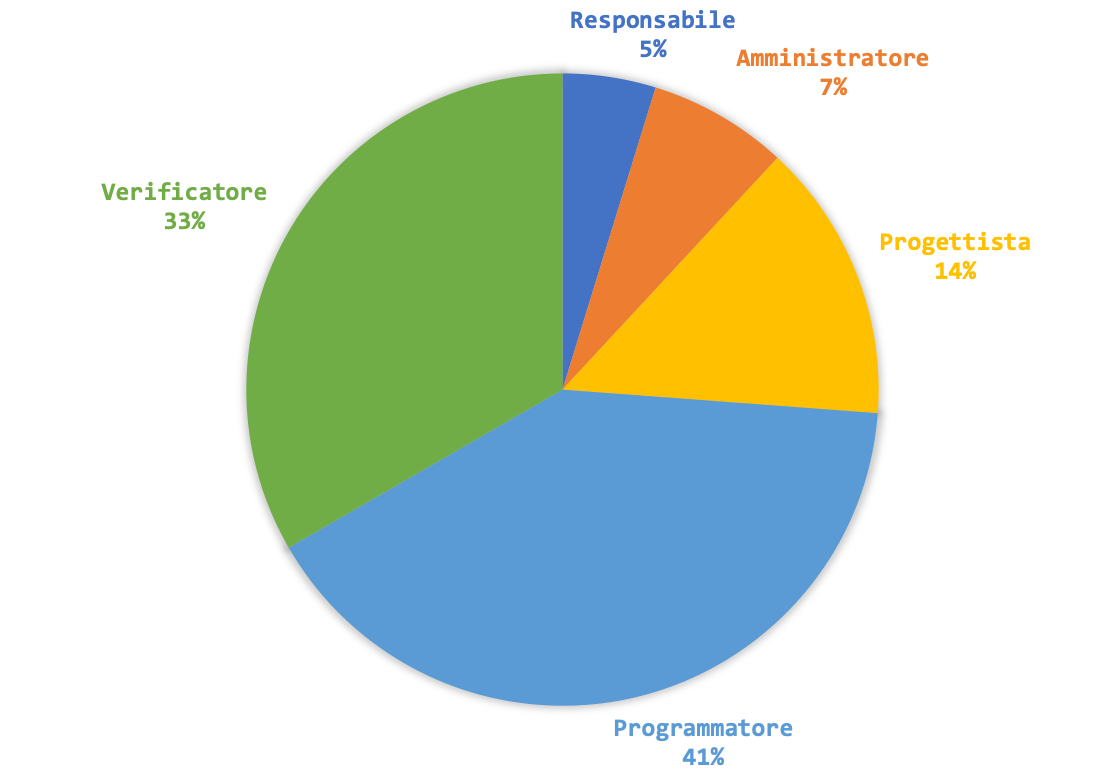
\includegraphics[width=0.8\linewidth]{./images/preventivo/incremento6-2.png}
			\caption{Grafico percentuale ore/ruolo incremento VI}
			\label{fig:grafico costi ruolo incremento VI}
		\end{figure}
		
		
		
		\subsection{Riepilogo ore totali}
			\subsubsection{Totale ore}
			\subparagraph{Totale prospetto orario }
			Riepilogo della distribuzione oraria di tutte le fasi:
			\rowcolors{2}{lightest-grayest}{white}
			\begin{longtable}{|c|c|c|c|c|c|c|c|}
				\hline
				\rowcolor{lighter-grayer}
				\textbf{Nome} & \textbf{Re} & \textbf{Am} & \textbf{An} & \textbf{Pg}  & \textbf{Pr}   & \textbf{Ve} & \textbf{Totale} \\
				\hline
				\endfirsthead
				
				\hline
				Giuseppe Vito Bitetti 		& 9 & 16 & 20 & 25 & 30 & 40 & 140\\
				\hline
				\hline
				Lorenzo Dei Negri			& 15 & 14 & 19 & 26 & 26 & 40 & 140\\
				\hline
				\hline
				Nicolò Frison				    & 13 & 10 & 21 &26 & 25 & 45 & 140\\
				\hline
				\hline
				Fouad Mouad 				 & 10 & 13 & 17 & 21 & 27 & 52 & 140\\
				\hline
				\hline
				Mariano Sciacco 			& 11 & 18 & 22 & 16 & 25 & 48 & 140\\
				\hline
				\hline
				Alessandro Tommasin    & 17 & 17 & 17 & 24 & 28 & 37 & 140\\
				\hline
				\hline
				Giovanni Vidotto 			 & 12 & 17 & 17 & 20 & 26 & 48 & 140\\
				\hline 
				\textbf{Totale}				 & 87 & 105 & 133 & 158 & 187 & 310 & 980\\
				\hline
				\caption{Tabella contenente un prospetto orario riepilogativo di tutti i periodi trattati in precedenza}
			\end{longtable}
			\pagebreak
			
			La tabella può essere riassunta nel seguente istogramma:
			\begin{figure}[H]
				\centering
				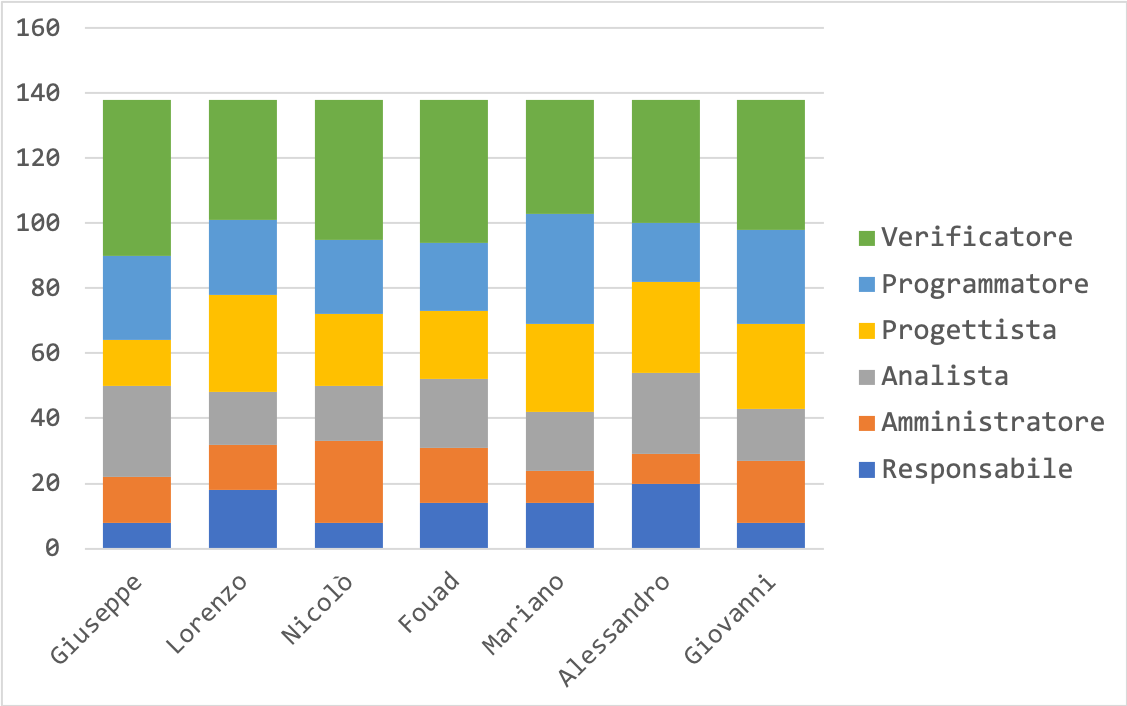
\includegraphics[width=0.8\linewidth]{./images/preventivo/totOre1.png}
				\caption{Grafico ore/ruolo componenti nel totale delle ore}
				\label{fig:grafico suddivione ruoli totale ore}
			\end{figure}
			
			\subparagraph{Totale prospetto economico}
			In base al prospetto orario, quello economico sarà il seguente: 
			
			\rowcolors{2}{white}{lightest-grayest}
			\begin{longtable}{|c|c|c|c|c|c|c|c|}
				\hline
				\rowcolor{lighter-grayer}
				\textbf{Ruolo} & \textbf{Ore} & \textbf{Costo in € } \\
				\hline
				\endfirsthead
				
				\hline
				Responsabile 	    & 87 & 2.610,00\\
				\hline 
				\hline
				Amministratore	  & 105 & 2.100,00\\
				\hline
				\hline
				Analista 				& 133 & 3.325,00\\
				\hline
				\hline
				Progettista 		  & 158 & 3.476,00\\
				\hline
				\hline
				Programmatore 	 & 187 & 2.805,00\\
				\hline
				\hline
				Verificatore 		  & 217 & 4.650,00\\
				\hline
				\textbf{Totale} 	& 735 & 18.966,00\\
				\hline
				\caption{Tabella contenente il prospetto economico in riferimento al prospetto orario nella tabella 14}
			\end{longtable}
			\pagebreak
			
			La tabella può essere riassunta nel seguente areogramma:
			\begin{figure}[H]
				\centering
				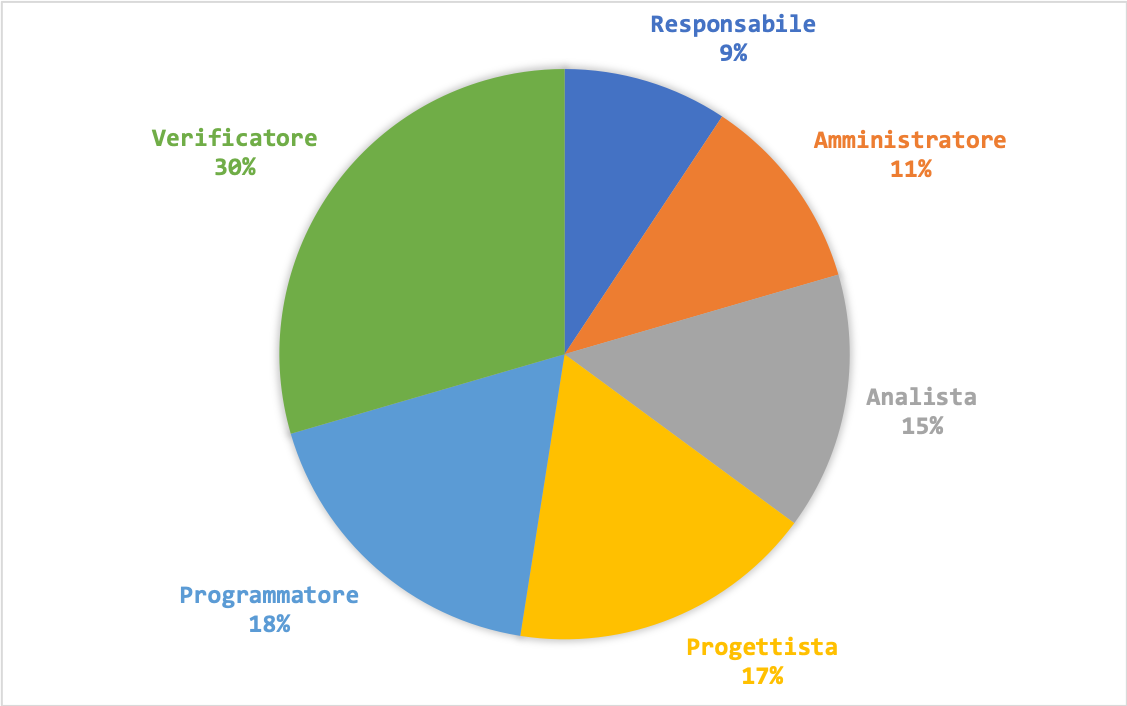
\includegraphics[width=0.8\linewidth]{./images/preventivo/totOre2.png}
				\caption{Grafico percentuale ore/ruolo nel totale delle ore}
				\label{fig:grafico costi ruolo fase totale ore}
			\end{figure}
		
			\subsubsection{Totale ore rendicontate}
				\subparagraph{Totale prospetto orario rendicontato}
				Riepilogo della distribuzione oraria delle fasi a carico del committente, escludendo quindi le fasi di analisi e consolidamento dei requisiti:
				
				\rowcolors{2}{lightest-grayest}{white}
				\begin{longtable}{|c|c|c|c|c|c|c|c|}
					\hline
					\rowcolor{lighter-grayer}
					\textbf{Nome} & \textbf{Re} & \textbf{Am} & \textbf{An} & \textbf{Pg}  & \textbf{Pr}   & \textbf{Ve} & \textbf{Totale} \\
					\hline
					\endfirsthead
					
					\hline
					Giuseppe Vito Bitetti 		& 9 & 7 & 6 & 25 & 30 & 38 & 105\\
					\hline
					\hline
					Lorenzo Dei Negri			& 7 & 9 & 6 & 26 & 26 & 31 & 105\\
					\hline
					\hline
					Nicolò Frison				    & 13 & 0 & 13 &26 & 25 & 28 & 105\\
					\hline
					\hline
					Fouad Mouad 				 & 8 & 6 & 6 & 21 & 27 & 37 & 105\\
					\hline
					\hline
					Mariano Sciacco 			& 3 & 18 & 7 & 16 & 25 & 36 & 105\\
					\hline
					\hline
					Alessandro Tommasin    & 6 & 17 & 3 & 24 & 28 & 7 & 105\\
					\hline
					\hline
					Giovanni Vidotto 			 & 10 & 10 & 9 & 20 & 26 & 30 & 105\\
					\hline 
					\textbf{Totale}				 & 56 &  67 & 50 & 158 & 187 & 217 & 735\\
					\hline
					\caption{Tabella contenente il prospetto orario preventivato a carico del committente}
				\end{longtable}
				\pagebreak
				
				La tabella può essere riassunta nel seguente istogramma:
				\begin{figure}[H]
					\centering
					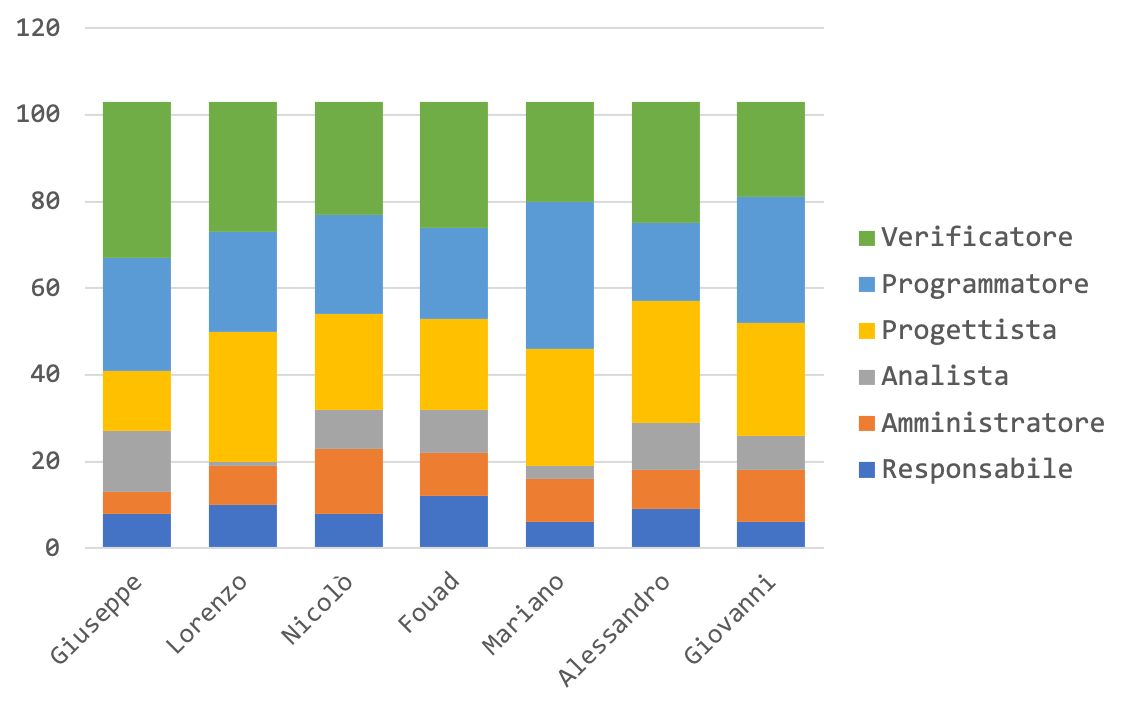
\includegraphics[width=0.8\linewidth]{./images/preventivo/totOreRed1.png}
					\caption{Grafico ore/ruolo componenti nel totale delle ore rendicontate}
					\label{fig:grafico suddivione ruoli totale ore rendicontete}
				\end{figure}
			
				\subparagraph{Totale prospetto economico rendicontato}
				In base al prospetto orario, quello economico sarà il seguente: 
				
				\rowcolors{2}{white}{lightest-grayest}
				\begin{longtable}{|c|c|c|c|c|c|c|c|}
					\hline
					\rowcolor{lighter-grayer}
					\textbf{Ruolo} & \textbf{Ore} & \textbf{Costo in €} \\
					\hline
					\endfirsthead
					
					\hline
					Responsabile 	    & 56 & 1.680,00\\
					\hline 
					\hline
					Amministratore	  & 67 & 1.340,00\\
					\hline
					\hline
					Analista 				& 50 & 1.250,00\\
					\hline
					\hline
					Progettista 		  & 158 & 3.476,00\\
					\hline
					\hline
					Programmatore 	 & 187 & 2.805,00\\
					\hline
					\hline
					Verificatore 		  & 217 & 3.255,00\\
					\hline
					\textbf{Totale} 	& 735 & 13.806,00\\
					\hline
					\caption{Tabella contenente il prospetto economico in riferimento al prospetto orario nella tabella 16}
				\end{longtable}
				\pagebreak
				
				La tabella può essere riassunta nel seguente areogramma:
				\begin{figure}[H]
					\centering
					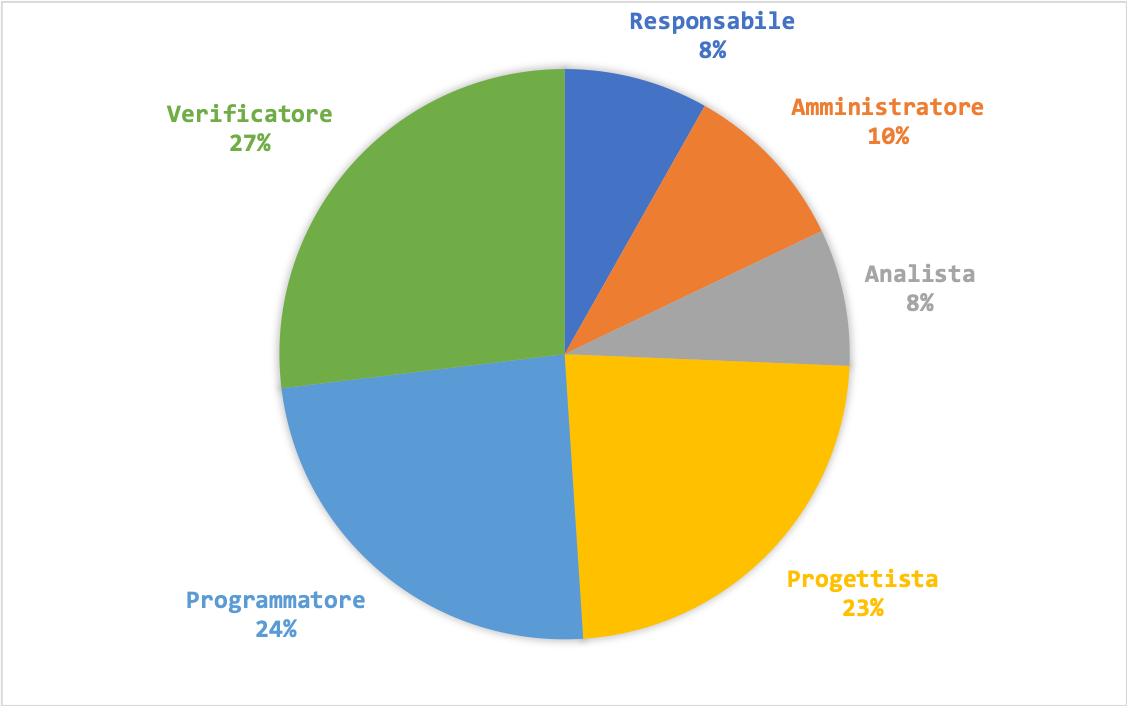
\includegraphics[width=0.8\linewidth]{./images/preventivo/totOreRed2.png}
					\caption{Grafico percentuale ore/ruolo nel totale delle ore rendicontate}
					\label{fig:grafico costi ruolo fase totale ore rendicontate}
				\end{figure}
			
			\subsection{Conclusioni}
				Il costo totale preventivato dal gruppo per lo sviluppo del progetto ammonta a 13.806,00 €.
				
				
		
	
	